\documentclass{article}

\usepackage[backend=biber]{biblatex}
\usepackage[utf8]{inputenc}
\usepackage[spanish]{babel}
\addbibresource{referencias.bib} 
\usepackage{hyperref}
\usepackage{graphicx}
\usepackage{listings}
\usepackage{xcolor}
\usepackage{float}
\usepackage{amsmath}
\usepackage{amssymb}
\usepackage{algorithm}
\usepackage{algpseudocode}
\usepackage{fancyhdr}
\usepackage{booktabs}

% ajustar margenes
\usepackage[margin=1in]{geometry}
\pagestyle{fancy}
\fancyhf{}
\rhead{\thepage}

\lstset { %
    language=C++,
    backgroundcolor=\color{black!5}, % set backgroundcolor
    basicstyle=\footnotesize,% basic font setting
}

\title{Analisis de Algoritmos \\ Tarea 1}
\date{18 de Abril 2025} 
\author{Cristóbal Figueroa Burgos, Joaquín San Martin Vargas, Camilo Tapia Correa}

\begin{document}

\maketitle


\section{Fuerza Bruta}

\subsection{Implementación}
  La implementación propuesta es la que se puede apreciar en la \textbf{Figura 1}.\\
  Se utilizo un Vector para almacenar el conjunto de puntos, se declara una variable minDistance encargada de almacenar el minimo valor, tiene 2 ciclos anidados que se encargan de recorrer todos los puntos del conjunto buscando la menor distacia en ellos.\\ En la seccion de correctitud se detalla el funcionamiento del algoritmo.
  \begin{figure}[H] % Usa [H] si estás usando el paquete float, para fijar la posición
    \centering
    \includegraphics[width=0.8\textwidth]{FuerzaBruta.png} % cambia el nombre
    \caption{Implementación fuerza bruta.}
    \label{fig:etiqueta_imagen}
\end{figure}
\begin{lstlisting}
\end{lstlisting}

\subsection{Correctitud}
Nuestro algoritmo recibe un conjunto $S = \{(X_i, Y_i)\} \mid i \in [0, n-1]$ de $n$ puntos en el plano y devuelve la mínima distancia entre ellos.

\vspace{1em}

\textbf{Input:} Conjunto $S = \{(X_i, Y_i)\} \mid i \in [0, n-1]$ de $n$ puntos en el plano.

\textbf{Output:} La distancia mínima entre puntos distintos del conjunto.

\vspace{1em}

\textbf{Main:}

\begin{algorithmic}
\State Declara una variable \texttt{minDistance} inicializándola con un número grande
\For{cada punto $(X_i, Y_i)$ en el conjunto $S$}
    \For{cada punto $(X_j, Y_j)$ tal que $j > i$}
        \State Calcular la distancia euclidiana entre $(X_i, Y_i)$ y $(X_j, Y_j)$
        \If{esta distancia es menor que \texttt{minDistance}}
            \State Reemplazar \texttt{minDistance} con esta distancia
        \EndIf
    \EndFor
\EndFor
\State Devolver \texttt{minDistance\\}
\end{algorithmic}
Para analizar la correctitud del algoritmo, utilizaremos \textbf{Invariante de ciclo}
\textbf{Antes del primer ciclo:\\}Al iniciar el primer ciclo minDistance almacena un valor tan grande que puede ser reemplazado con cualquier distancia.\\
\textbf{En el ciclo:\\}
En cada ciclo, se comparan 2 puntos, si su distancia es menor a la que esta almacenada en minDistance, actualizara esta variable.
Esto garantiza que minDistance siempre mantenga la menor distancia encontrada.\\
\textbf{Al salir del ciclo:\\}
Al finalizar el ciclo habremos revisado todas las posibles combinaciones de pares de puntos en S, por lo que minDistance almacenara
la minima distancia entre cualquier par de puntos en S.




\subsection{Complejidad Computacional}
El primer ciclo del código propuesto recorre $i$ desde $0$ hasta $n - 1$, con lo que se realizan $n - 1$ iteraciones. Luego, el segundo ciclo interno comienza con $j = i + 1$, por lo tanto, para la primera iteración del primer ciclo se hacen $n - 1$ comparaciones, luego $n - 2$, luego $n - 3$, y así sucesivamente, hasta llegar a $1$.\\ Esto se puede expresar como la suma:
\[
(n - 1) + (n - 2) + (n - 3) + \cdots + 2 + 1 = \frac{(n - 1) \cdot n}{2}
\]\\Por lo tanto, la complejidad del algoritmo es $\mathcal{O}(n^2)$.

  
\section{Dividir para Vencer}
    1\subsection{Diseño}
El diseño de \textit{Divide and Conquer} se basa en el algoritmo de \textbf{GeeksforGeeks}\cite{geeks2023}. El Algoritmo es el siguiente:\\\textbf{\\Input:} Conjunto $S = \{(X_i, Y_i)\} \mid i \in [0, n-1]$ de $n$ puntos en el plano.\\\textbf{Output:} La distancia mínima entre puntos distintos del conjunto.\\
\\Primero, el algoritmo ordena los puntos del conjunto $S$ según su coordenada $X$. 
Una vez ordenado, se busca el punto medio y se divide el conjunto en dos subconjuntos:

\begin{itemize}
    \item $P_{\text{izq}} = \{(X_0, Y_0),\ldots, (X_{\lfloor n/2 \rfloor - 1}, Y_{\lfloor n/2 \rfloor - 1})\}$
    \item $P_{\text{der}} = \{(X_{\lfloor n/2 \rfloor}, Y_{\lfloor n/2 \rfloor}),\ldots, (X_{n-1}, Y_{n-1})\}$
\end{itemize}
Luego, de manera recursiva, se busca la distancia mínima en los conjuntos $P_{\text{izq}}$ y $P_{\text{der}}$:

\[
d = \min(d_{\text{izq}}, d_{\text{der}})
\]

Con esto, sabemos que la distancia mínima del conjunto completo debe ser menor o igual a $d$.
\begin{figure}[H] % Usa [H] si estás usando el paquete float, para fijar la posición
    \centering
    \includegraphics[width=0.6\textwidth]{mindis.png} % cambia el nombre
    \caption{Division del Conjunto.}
    \label{fig:etiqueta_imagen}
\end{figure}
\begin{lstlisting}
\end{lstlisting}
Ahora, consideramos los pares que están en \textit{\textbf{la frontera}}, es decir, aquellos en los que un punto pertenece a la parte izquierda y otro a la derecha.
Imaginando una línea vertical que pasa por $X_{\lfloor n/2 \rfloor}$ como se aprecia en la \textbf{Figura 3}, analizamos los pares de puntos cuya coordenada $x$ está a una distancia menor que $d$ de esta línea.

\vspace{1em}
 \begin{figure}[H] % Usa [H] si estás usando el paquete float, para fijar la posición
    \centering
    \includegraphics[width=0.6\textwidth]{closepair.png} % cambia el nombre
    \caption{Frontera del conjunto dividido.}
    \label{fig:etiqueta_imagen}
\end{figure}
\begin{lstlisting}
\end{lstlisting}

Para los puntos en la frontera, primero los ordenamos por su coordenada $Y$. Luego, para cada punto, lo comparamos con los siguientes $6$ o $7$ puntos más cercanos a lo largo del eje $Y$.
Esto se debe a que, al ordenar por $Y$, los puntos en la franja vertical de ancho $2d$ están distribuidos en un área donde, geométricamente, no pueden existir más de 6 puntos a menos de $d$ de distancia entre sí. Esta propiedad se basa en la densidad máxima de puntos en un rectángulo de dimensiones $d \times d$.

\vspace{1em}

Finalmente, la distancia mínima entre los puntos del conjunto $S$ será:

\[
\min(d_{\text{izq}}, d_{\text{der}}, d_{\text{frontera}})
\]



\subsection{Correctitud}
Demostraremos la correctitud del Algoritmo \textit{divide and conquer} para encontrar la distancia mínima entre dos puntos funciona correctamente usando inducción matemática.
\subsection*{Hipótesis}
Sea $P(n)$: “El algoritmo encuentra correctamente la distancia mínima entre dos puntos distintos de un conjunto de $n$ puntos en el plano”.
\subsection*{Caso base: $n = 2$ o $n = 3$}
Cuando hay solo 2 o 3 puntos, el algoritmo compara todas las posibles distancias directamente.  
En este caso, claramente devuelve la distancia mínima de forma correcta.
Por lo tanto, $P(2)$ y $P(3)$ son verdaderos.
\subsection*{Paso inductivo}
Supongamos que el algoritmo funciona correctamente para todo conjunto de $k$ puntos, con $k \leq n$.  
Queremos probar que también funciona para un conjunto de $n+1$ puntos.
El algoritmo:

\begin{itemize}
    \item Ordena los puntos por coordenada $x$.
    \item Divide el conjunto en dos mitades.
    \item Aplica el algoritmo recursivamente en cada mitad. Por la hipótesis inductiva, cada mitad devuelve la distancia mínima correcta.
    \item Luego compara los puntos cercanos a la línea divisoria (frontera), y revisa solo los que pueden estar a una distancia menor que la mínima encontrada hasta ahora.
\end{itemize}

Finalmente, devuelve el mínimo entre:

\begin{itemize}
    \item la distancia mínima en la mitad izquierda,
    \item la distancia mínima en la mitad derecha,
    \item y las distancias entre puntos cercanos a la frontera.
\end{itemize}

Esto asegura que el resultado es correcto también para $n+1$ puntos.

\subsection*{Conclusión}

Por inducción matemática, el algoritmo funciona correctamente para cualquier cantidad de puntos $n \geq 2$.

\subsection{Complejidad Computacional}
El algoritmo en sencillos pasos hace lo siguiente.\\ primero
\begin{enumerate}
    \item Ordena todos los puntos del conjunto por su coordenada X,
    \item luego divide el conjunto en dos mitades, despues
    \item recursivamente encuentra la distancia en las dos mitades
    \item combina los resultados considerando los puntos cercanos a la frontera
    \item Comparar todos los pares en la frontera dentro de una distancia d del eje divisorio
    \item y finalmente, ordenar esa franja por coordenada Y e compara solo hasta 6-7 vecinos siguientes.
\end{enumerate}
El ordenar los puntos por su coordenada x tiene complejidad $\mathcal{O}(n \log n)$.


  
\section{Implementación}

Ambos algoritmos fueron implementados y testeados en lenguaje C++. A continuación, se presentan fragmentos relevantes del código:

\subsection{Fuerza Bruta}

\begin{lstlisting}[language=C++]
double minDist_BF(std::vector<std::pair<double, double>> &dots) {
    double minDistance = std::numeric_limits<double>::max();
    
    for (size_t i = 0; i < dots.size(); i++) {
        for (size_t j = i+1; j < dots.size(); j++) {
            double distance = calculateDistance(dots[i], dots[j]);
            if (distance <= minDistance) {
                minDistance = distance;
            }
        }
    }
    return minDistance;
}
\end{lstlisting}

\subsection{Divide y Vencerás}

\begin{lstlisting}[language=C++]
double minDist_DQ(std::vector<std::pair<double, double>> &dots) {
    // Ordenar los puntos por coordenada x
    std::sort(dots.begin(), dots.end(), compX);
    
    // Llamar a la funcion recursiva
    return minDist(dots, 0, dots.size());
}
double minDist(std::vector<std::pair<double, double>> &dots, int left, int right) {
    // Caso base: si hay 2 o menos puntos, usamos fuerza bruta
    if (right - left <= 3) {
        // Implementacion del caso base omitida por brevedad
    }   
    // Dividir el conjunto de puntos en dos mitades
    int mid = (left + right) / 2;
    
    // Calcular la distancia minima en las dos mitades
    double dIzq = minDist(dots, left, mid);
    double dDer = minDist(dots, mid, right);
    
    // Tomar la minima distancia entre las dos mitades
    double d = std::min(dIzq, dDer);
    
    // Considerar puntos en la franja central
    // Implementacion omitida por brevedad
    
    return minDistCentro(centro, d);
}
\end{lstlisting}
  
\section{Análisis Experimental}

\subsection{Diseño}

Diseñe un análisis experimental calculando los tiempos de ejecución en nanosegundos de sus dos soluciones para un conjunto de $n$ puntos cuyas coordenadas enteras están elegidas al azar en un cuadrado de $100\times100$, variando la cantidad $n$ de puntos entre las potencias de dos de $2^3=8$ a $2^{9}=512$.

\subsection{Realización}
\begin{table}[H]
\centering
\caption{Tiempos de ejecución de los algoritmos (en nanosegundos)}
\begin{tabular}{ccccc}
\toprule
\multirow{2}{*}{$n$} & \multicolumn{2}{c}{Fuerza Bruta} & \multicolumn{2}{c}{Divide y Vencerás} \\
\cmidrule(lr){2-3} \cmidrule(lr){4-5}
& $t_{\text{mean}}$ & $t_{\text{stdev}}$ & $t_{\text{mean}}$ & $t_{\text{stdev}}$ \\
\midrule
8 & 4910.53 & 3506.34 & 8999.72 & 2790.8 \\
16 & 12288.5 & 1468.18 & 15573.4 & 2395.99 \\
32 & 42171.3 & 5123.67 & 29484.7 & 4839.82 \\
64 & 149633 & 24830.6 & 65055.3 & 11696.5 \\
128 & 618875 & 90648.2 & 147532 & 25404.6 \\
256 & $2.64631 \times 10^6$ & 540132 & 325615 & 44086.6 \\
512 & $1.00899 \times 10^7$ & 924821 & 678608 & 102115 \\
\bottomrule
\end{tabular}
\end{table}
    
\section{Mejora}
Observando el tiempo de ejecución para valores grandes de $n$, proponga y evalúe una versión trivialmente mejorada de los dos algoritmos.

\section{Gráfico} Construya un gráfico que muestre cómo varían los tiempos de ejecución de sus cuatros soluciones en nanosegundos, variando la cantidad $n$ de puntos entre las potencias de dos de $2^3=8$ a $2^9=512$.

\begin{figure}[H]
\centering
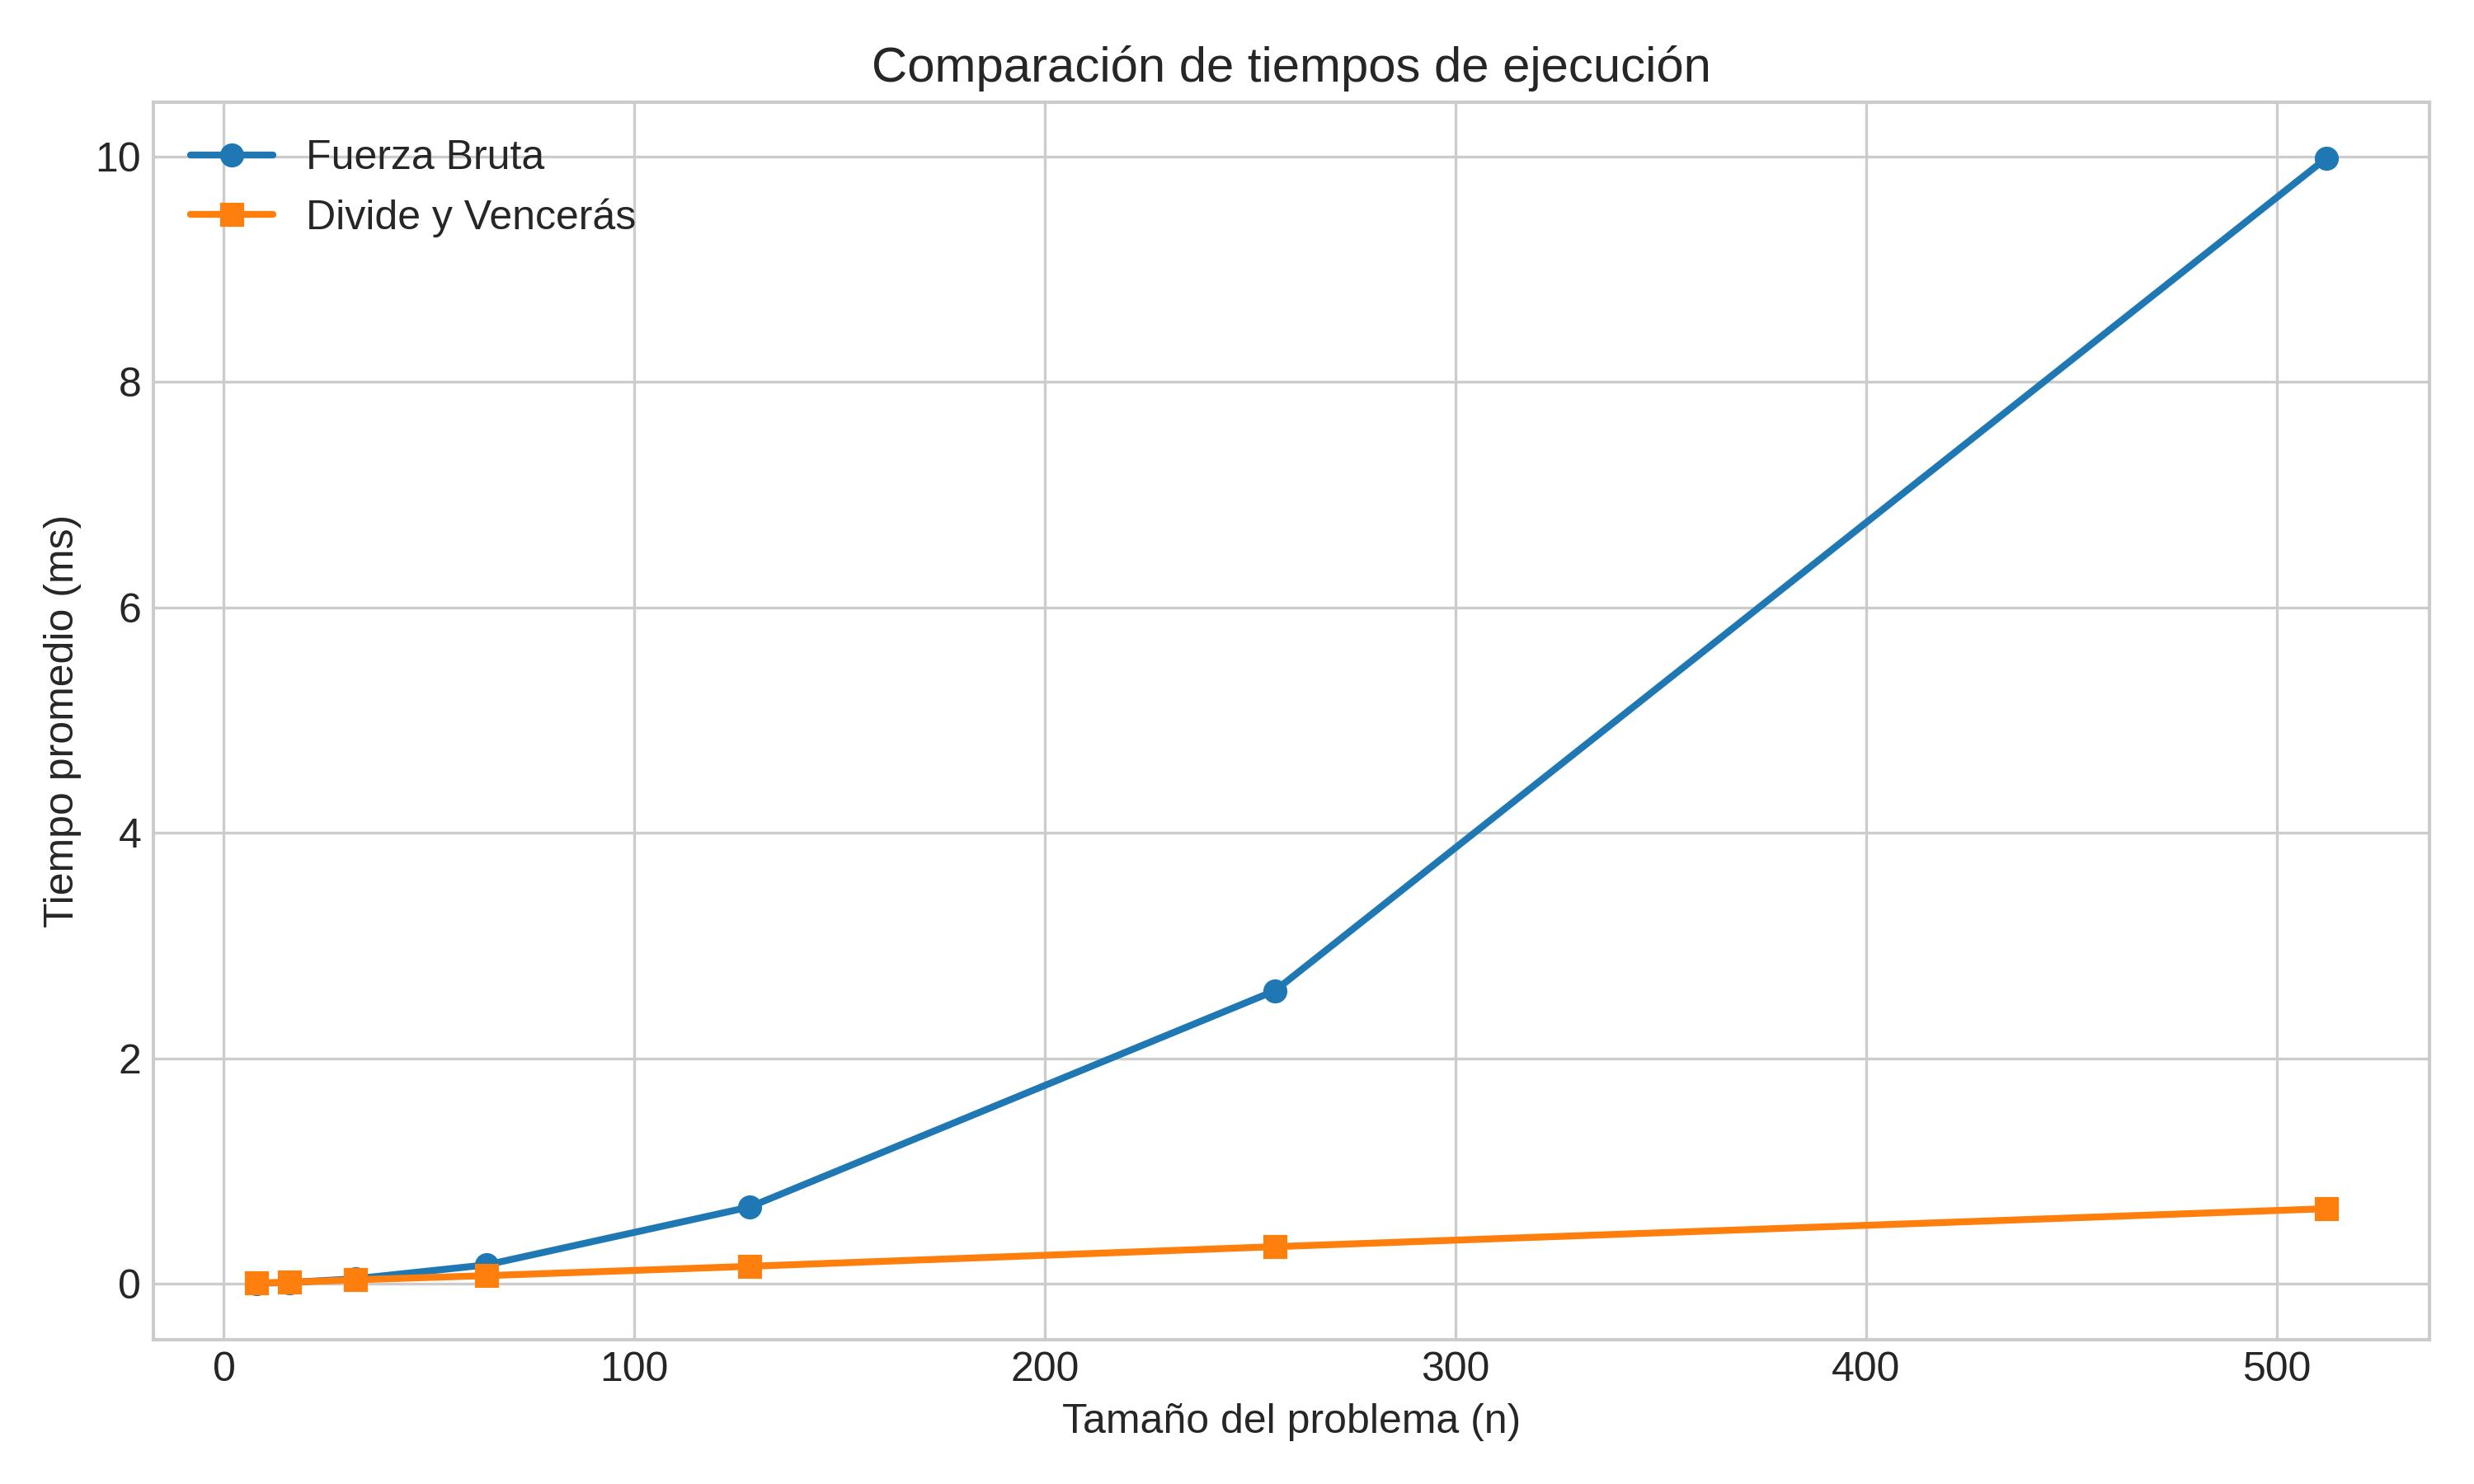
\includegraphics[width=0.8\textwidth]{normal_comparison.jpg}
\caption{Comparación de tiempos de ejecución}
\end{figure}

Como se puede observar en la gráfica, para tamaños de entrada pequeños ($n \leq 16$), el algoritmo de Fuerza Bruta es ligeramente más rápido que el de Divide y Vencerás. Sin embargo, a medida que el tamaño del problema aumenta, el algoritmo de Divide y Vencerás muestra un rendimiento significativamente mejor.

\subsection{Análisis en escala logarítmica}

\begin{figure}[H]
\centering
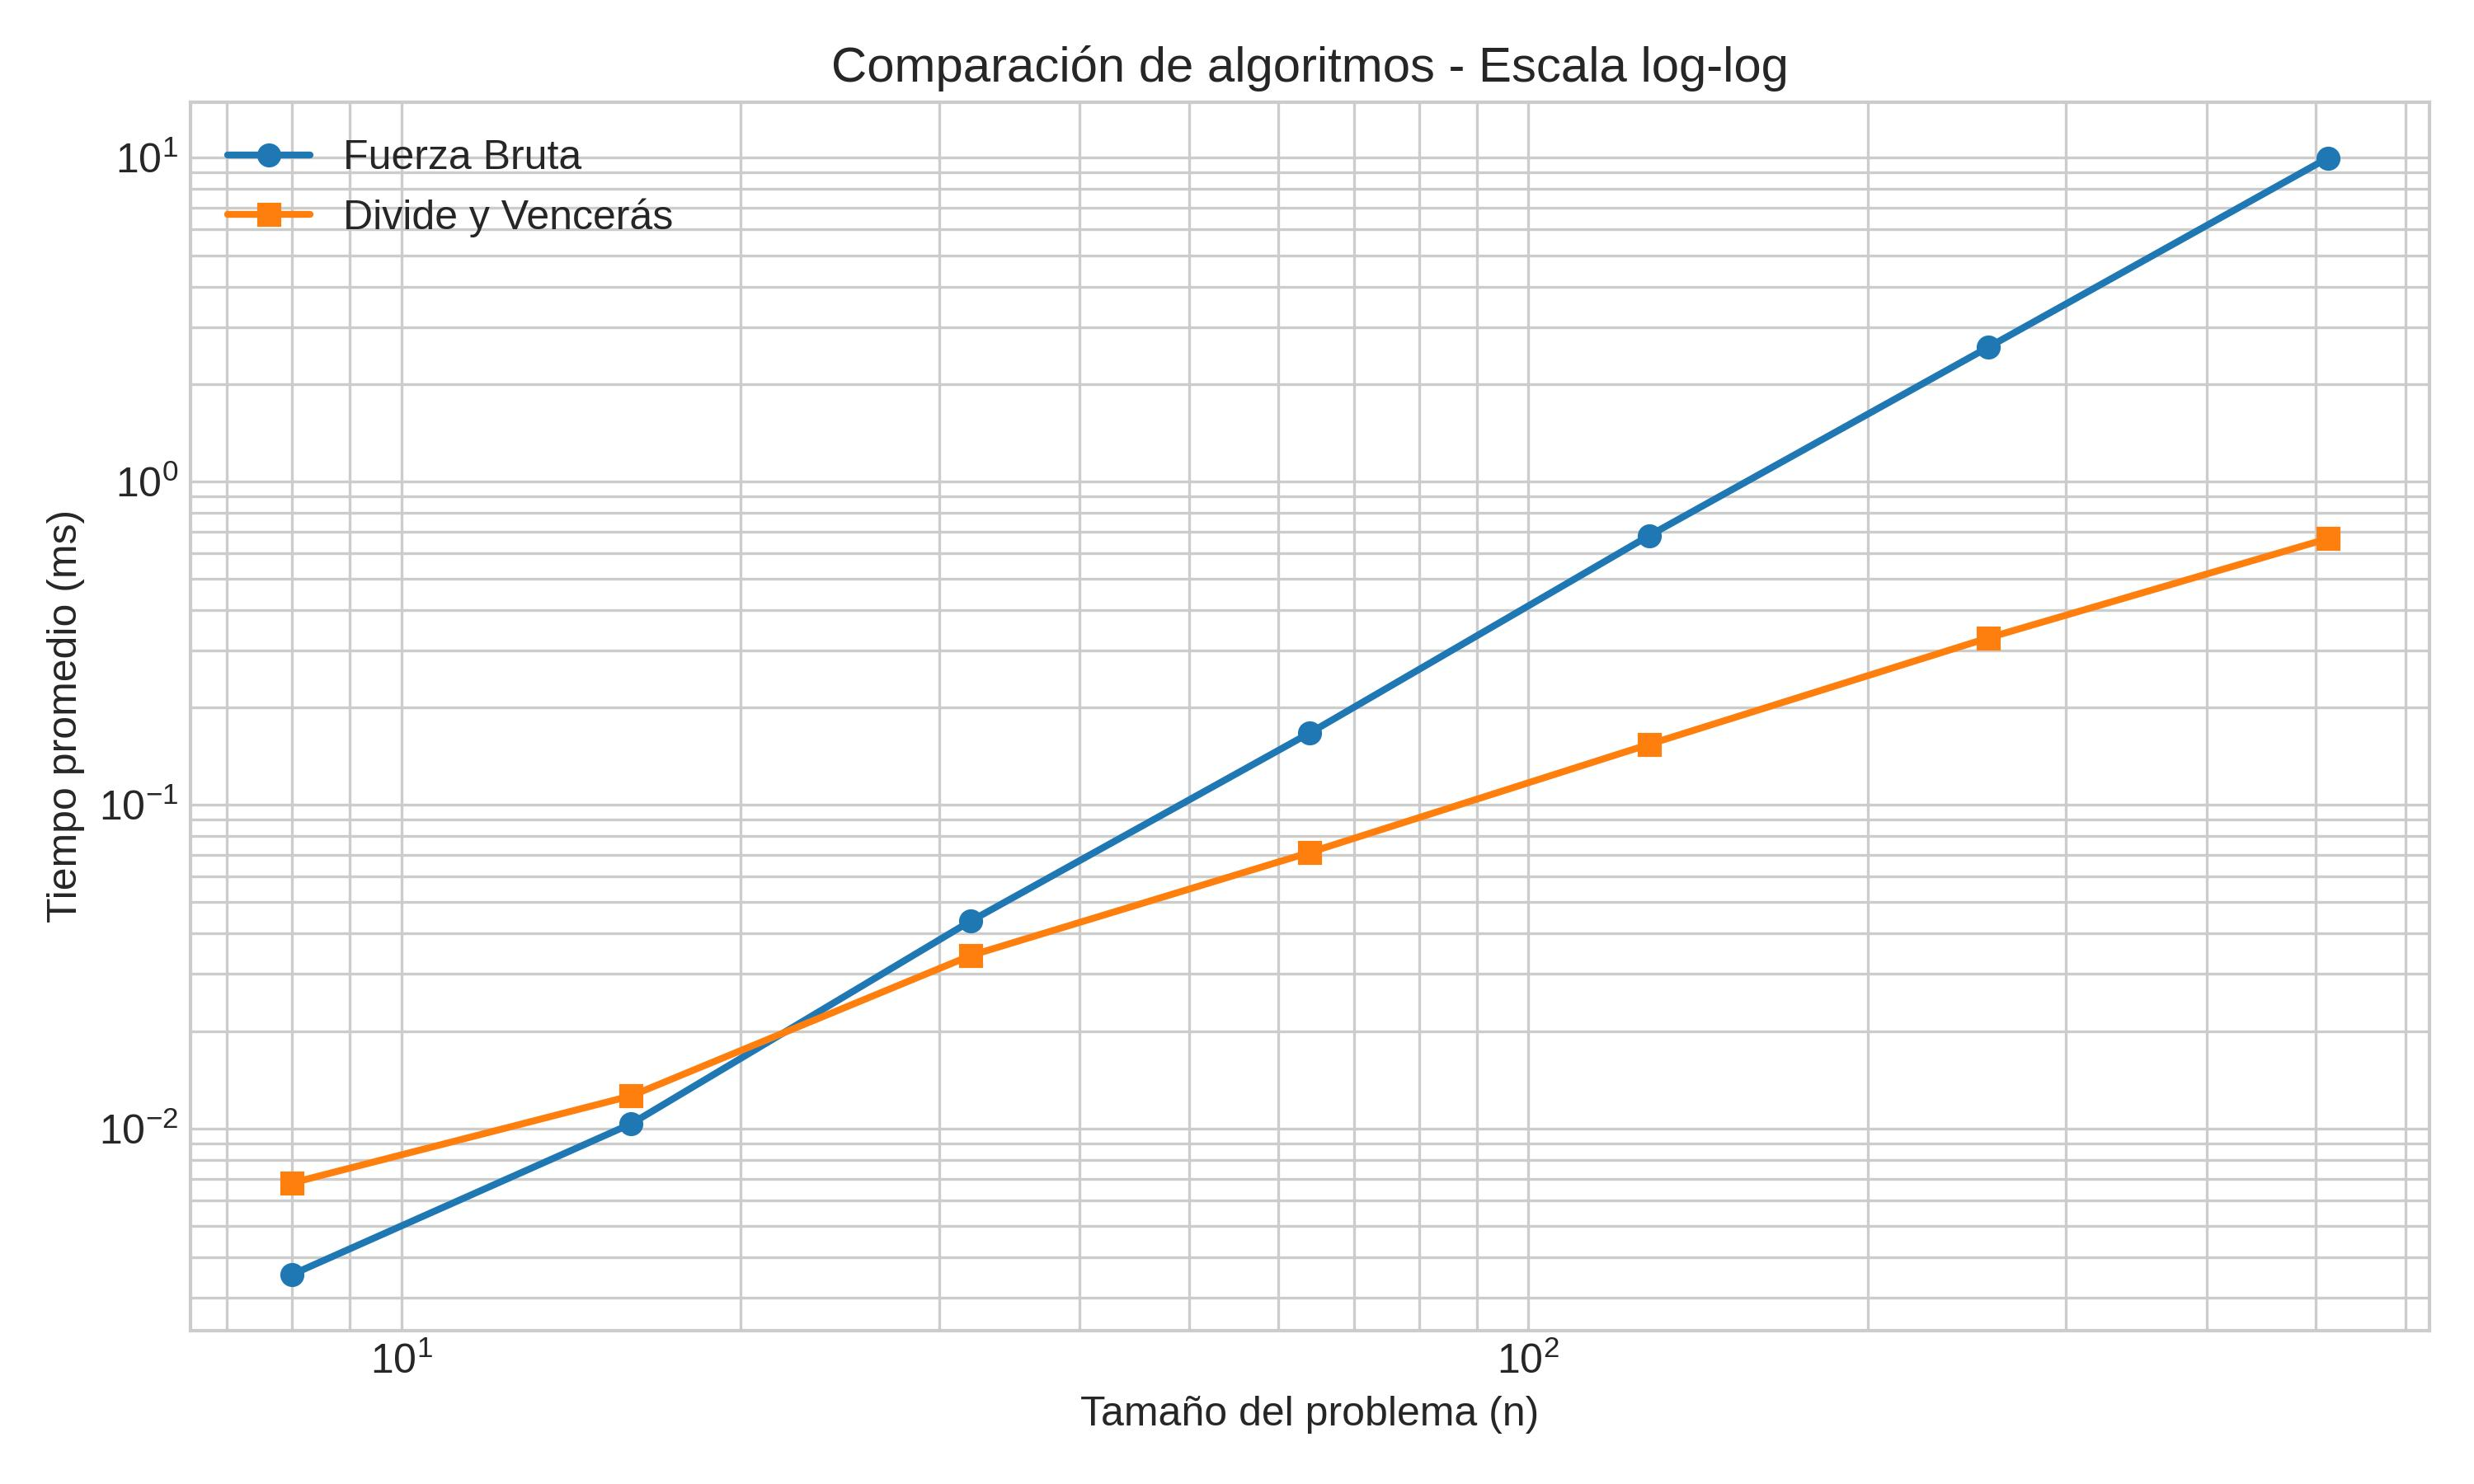
\includegraphics[width=0.8\textwidth]{log_log_comparison.jpg}
\caption{Comparación de algoritmos - Escala log-log}
\end{figure}

La representación en escala logarítmica nos permite visualizar mejor el comportamiento asintótico de ambos algoritmos. Se aprecia claramente que la pendiente de la curva de Fuerza Bruta es mayor que la de Divide y Vencerás, lo que confirma la complejidad teórica de $O(n^2)$ y $O(n \log n)$ respectivamente.

\subsection{Speedup}

\begin{figure}[H]
\centering
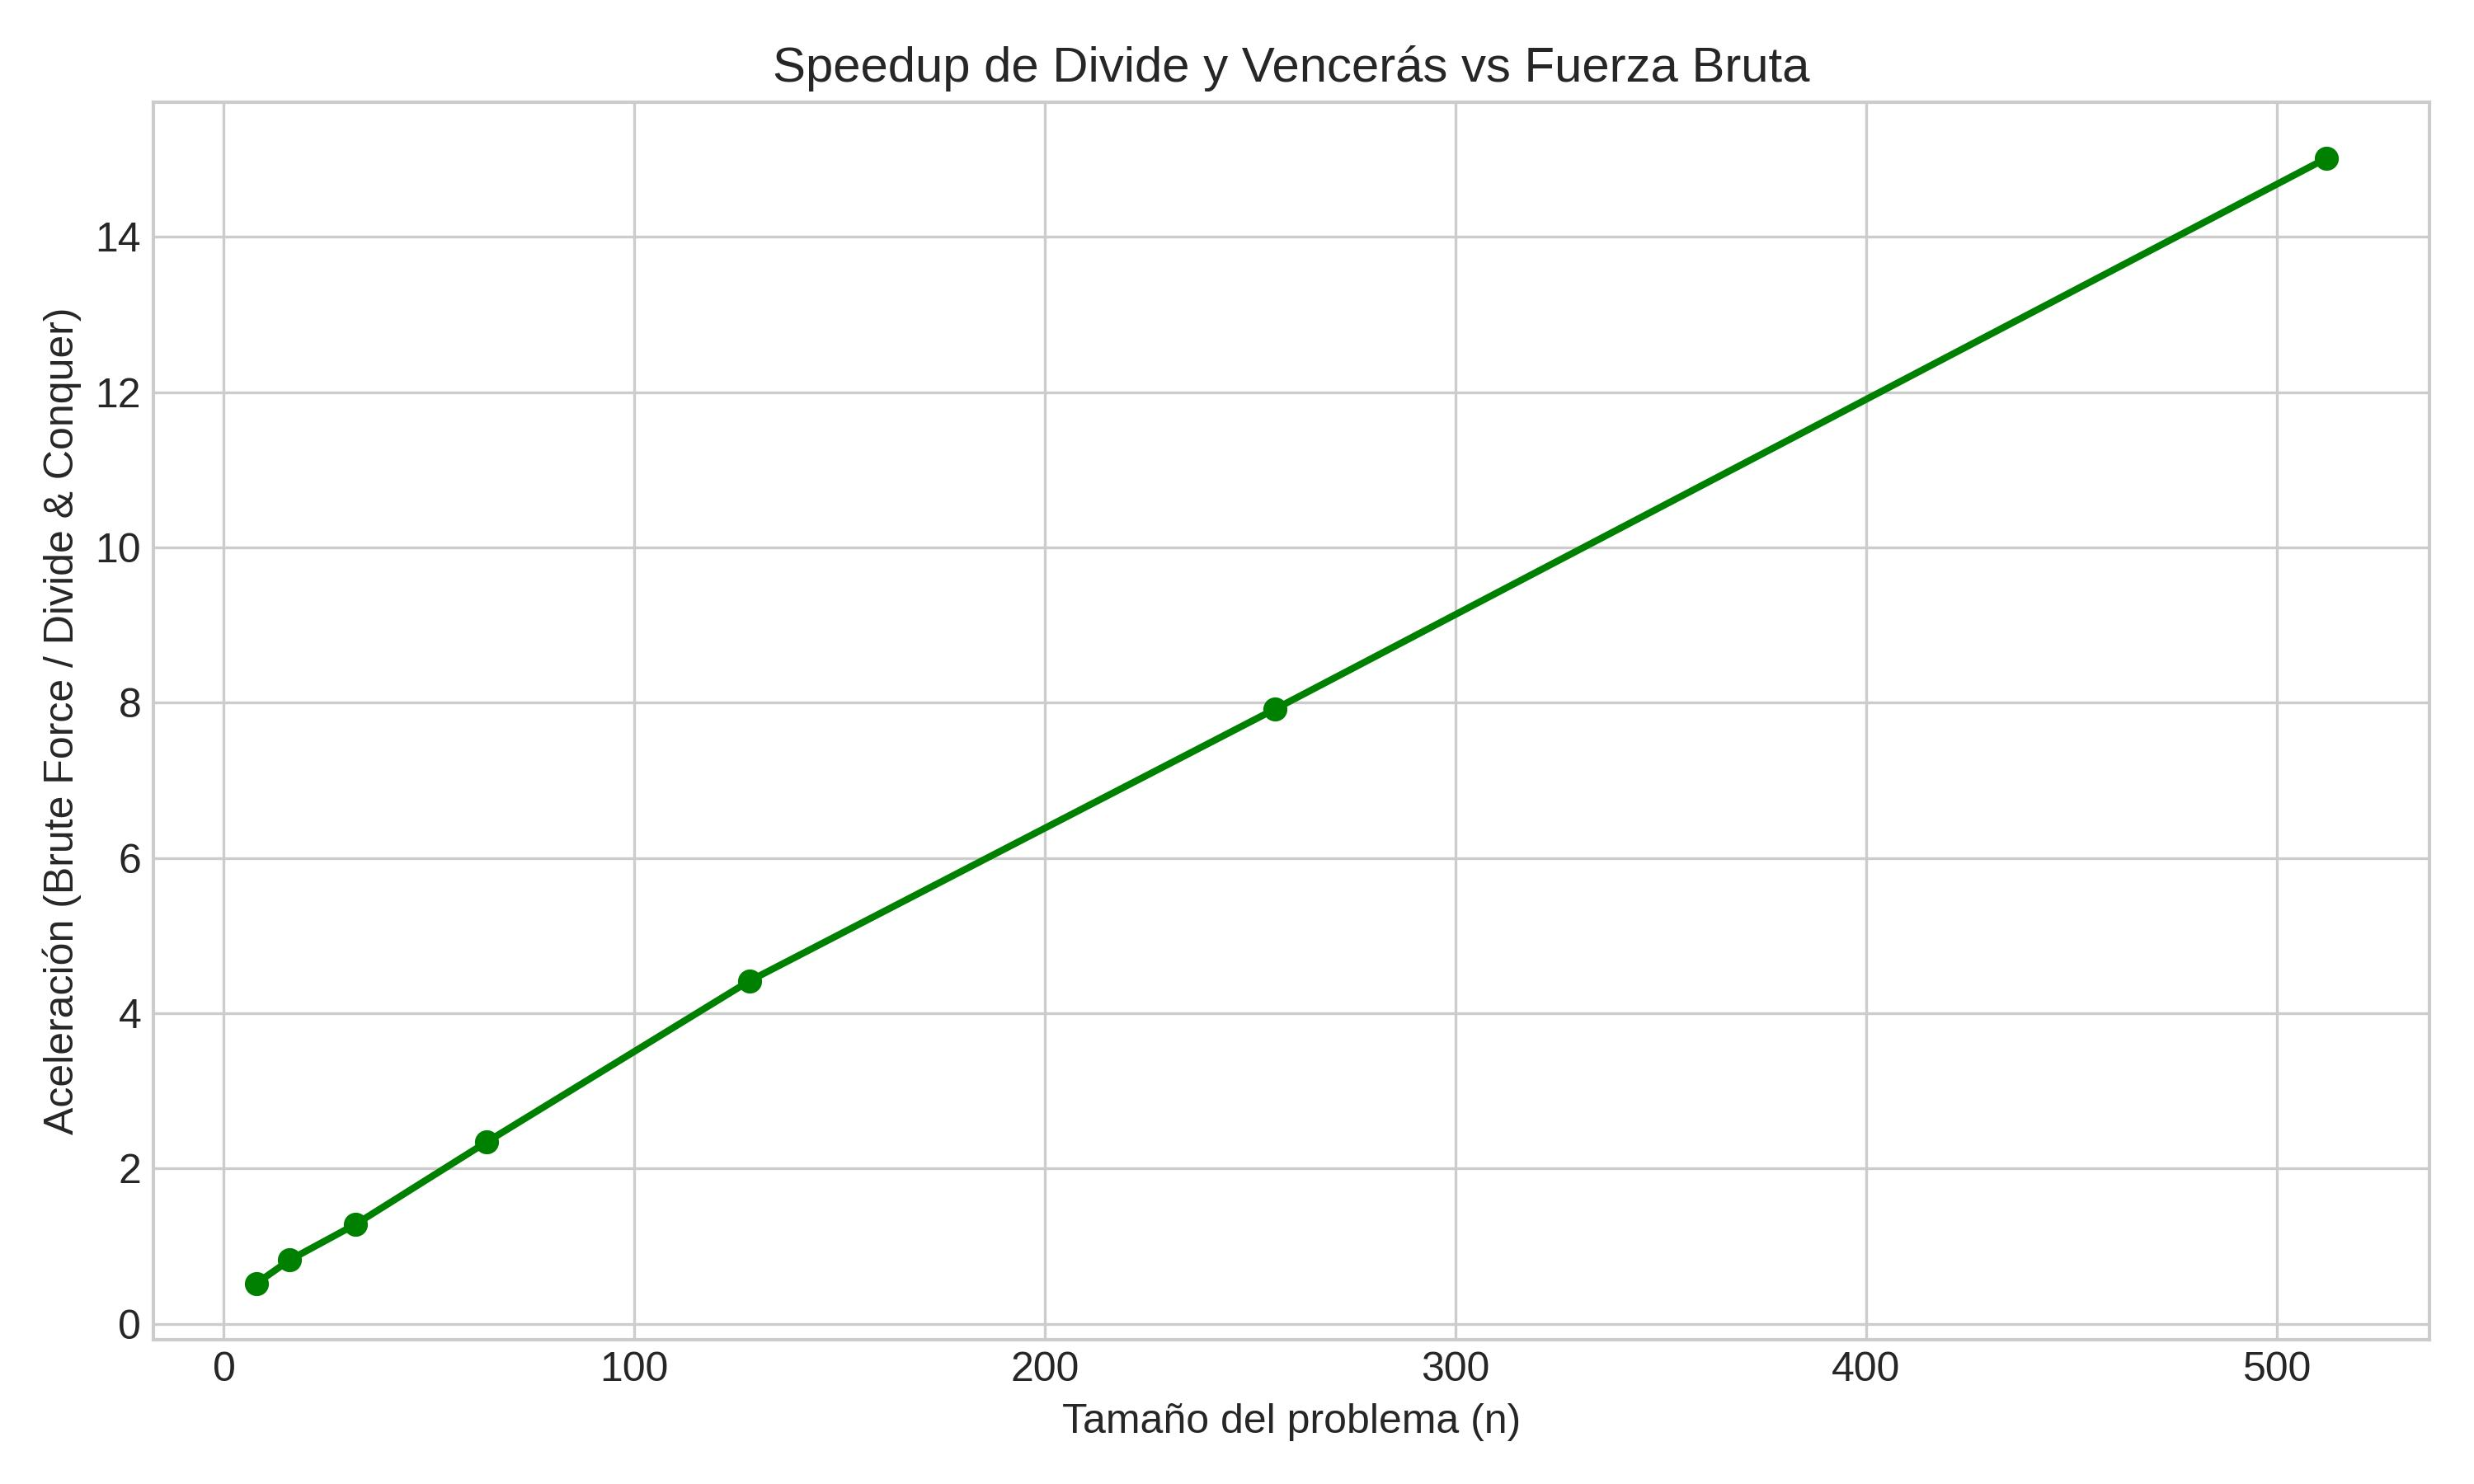
\includegraphics[width=0.8\textwidth]{speedup.jpg}
\caption{Speedup de Divide y Vencerás vs Fuerza Bruta}
\end{figure}

El speedup (aceleración) obtenido al utilizar Divide y Vencerás en lugar de Fuerza Bruta aumenta significativamente con el tamaño del problema. Para $n = 512$, el algoritmo de Divide y Vencerás es aproximadamente 15 veces más rápido que el de Fuerza Bruta.

\subsection{Variabilidad de los tiempos}

\begin{figure}[H]
\centering
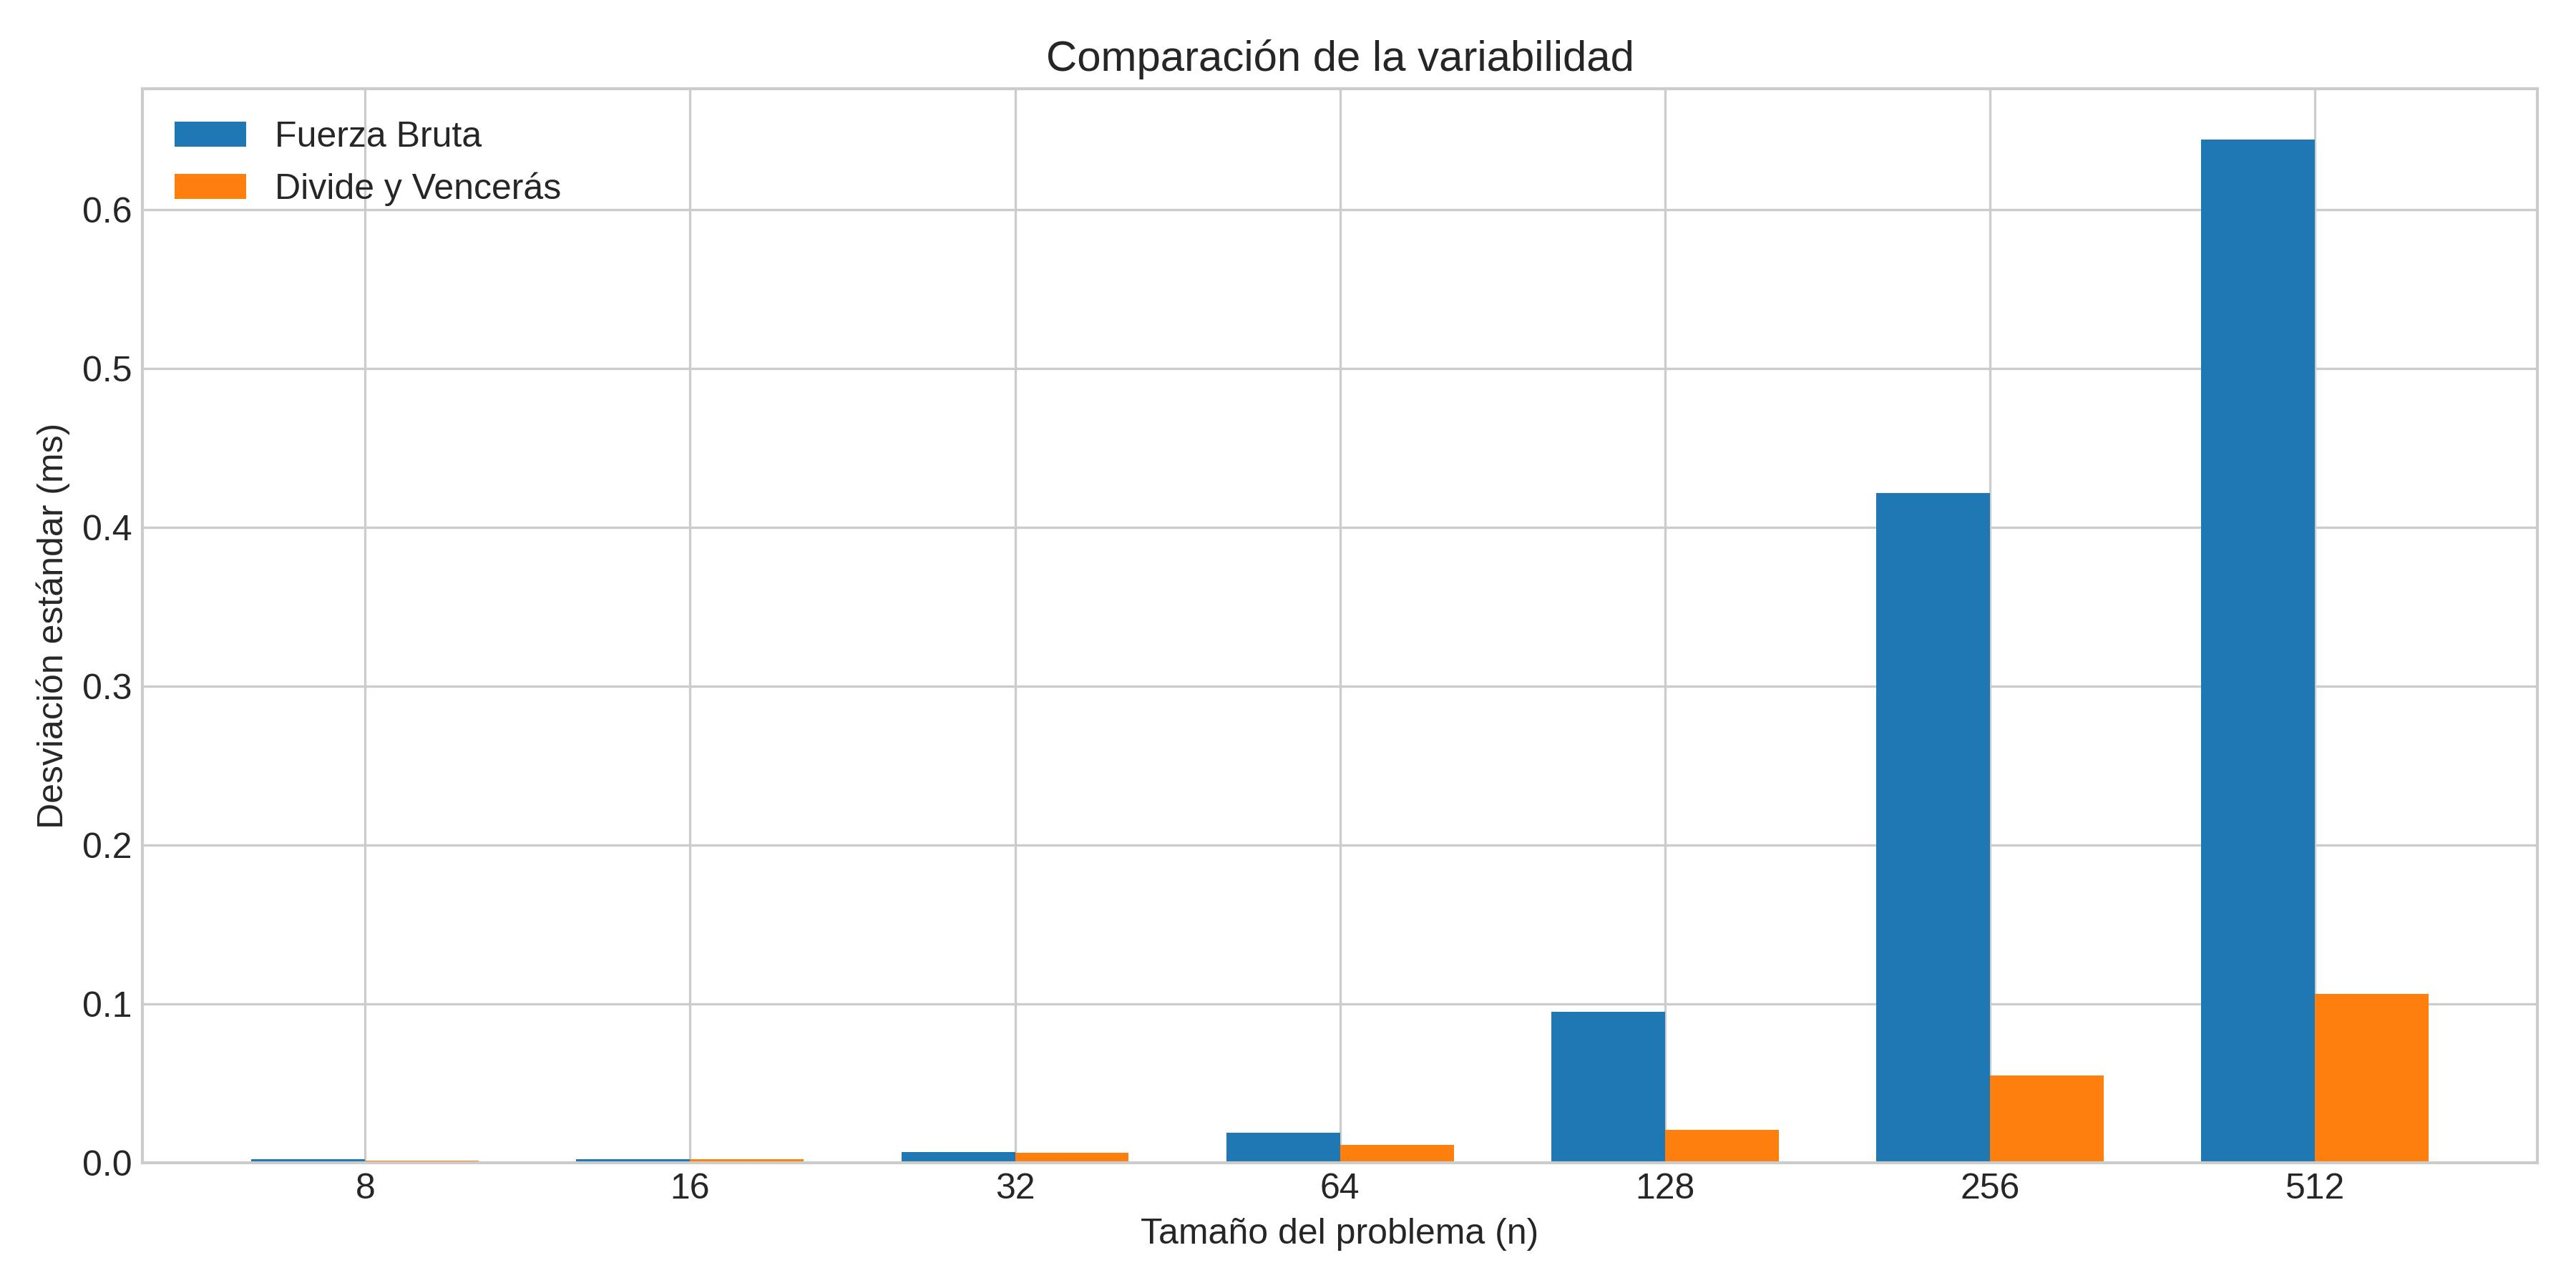
\includegraphics[width=0.8\textwidth]{stdev_comparison.jpg}
\caption{Comparación de la variabilidad}
\end{figure}

La desviación estándar de los tiempos de ejecución es considerablemente menor en el algoritmo de Divide y Vencerás, lo que indica que este algoritmo ofrece un rendimiento más estable y predecible en comparación con el de Fuerza Bruta.


\printbibliography
\end{document}
